\documentclass{article}

\date{10 Mars 2024}
\usepackage[nb-sem=20, auteurs={Hugo Vangilluwen, George Ober, Kylian Boyet}]{../kholles}

\begin{document}
\maketitle

\begin{question_kholle}
  [{\begin{equation}
    \K[X] ^\times = \left\{ \lambda X^0, \lambda \in \K^* \right\}
  \end{equation}}]
  {Éléments inversibles de l'anneau $\K[X]$}
  
  Soit P un élément inversible de $\K[X]$.
  Alors $\exists Q \in \K[X] : P \cdot Q = Q \cdot P = 1_{\K[X]}$.
  En prenant les degrés des polynômes, $\text{deg } P + \text{deg } Q = 0$. \\
  Or $\text{deg } : \K[X] \rightarrow \N$ donc $\text{deg } P = \text{deg } Q = 0$.
  Donc $\exists \lambda \in \K^* : P = \lambda$. \\
  Ainsi $\K[X]^\times \subset \left\{ \lambda X^0, \lambda \in \K^* \right\}$.
  
  Soit $\lambda \in \K^*$. Considérons $P = \lambda$.
  Posons $Q = \lambda^{-1}$ (car \K est un corps). $P \cdot Q = \lambda \lambda^{-1} = 1$ et $Q \cdot P = \lambda^{-1} \lambda = 1$ donc $P$ est inversible. Ainsi $\left\{ \lambda X^0, \lambda \in \K^* \right\} \subset \K[X]^\times$.
\end{question_kholle}

\begin{question_kholle}
  [Le problème d'interpolation de Lagrange est, pour $n \in \N$ avec $a \in \K^{n+1}$ et $b \in \K^{n+1}$, l'ensemble des polynômes passant par tous les points de coordonnée $(a_i, b_i)$. C'est-à-dire l'ensemble des {$P \in \K[X]$} vérifiant :
  {\begin{equation}
    \forall i \in [\![0;n]\!], P(a_i) = b_i
  \end{equation}}
  Il existe une unique solution $P$ de degré $\leqslant n$ au problème d'interpolation de lagrange, et elle s'exprime de la manière suivante en posant
  \begin{equation}
    L_{i} = \prod_{\substack{j=0\\j \neq i}}^{n} \frac{X - a_{j}}{a_{i} - a_{j}}
  \end{equation}
  \begin{equation}
    P = \sum_{i=0}^{n}b_{i}L_{i}
  \end{equation}]
  {Théorème d'interpolation de lagrange}
  
  \begin{itemize}
    \item Unicité
    
    Supposons qu'il existe $(P, Q) \in \mathbb{K}_n[X]^{2}$ solutions du problème d'interpolation.
    
    Alors $\forall i \in [ \! [ 0, n ] \!], \tilde{P}(a_{i}) = \tilde{Q}(a_{i}) = b_{i}$
    
    Posons $H = P - Q$, alors, $\forall i \in [ \! [ 0, n ] \!], \tilde{H}(a_{i}) = \tilde{P}(a_{i}) - \tilde{Q}(a_{i}) = 0$.
    
    De plus, $\deg H = \deg(P-Q) \leqslant \max \left\{ \deg P, \deg Q \right\}$
    
    Donc $H$ est un polynôme de degré $\leqslant n$ avec $\lvert [ \! [ 0, n ] \!] \rvert = n+1$ racines.
    
    Donc $H$ est le polynôme nul.
    \item Existence
    Soit $i \in [ \! [ 0, n ] \!]$ fq
    Notons $L_{i}$ une solution de degré $\leqslant n$ au problème $Pb_{i}$ suivant:
    $$
    (Pb_i)
    \left\{ \begin{array}{ll}
      \tilde{P}(a_{0}) = 0   \\
      \vdots                 \\
      \tilde{P}(a_{i-1}) = 0 \\
      \tilde{P}(a_{i}) = 1   \\
      \tilde{P}(a_{n}) = 0   \\
      \vdots                 \\
      \tilde{P}(a_{n}) = 0
    \end{array} \right.
    $$
    On remarque que $(a_{0},\dots ,a_{i-1}, a_{i+1},\dots, a_{n})$ sont $n$ racines deux à deux distinctes de $L_{i}$. Or $L_{i}$ est de degré $\leqslant n$ et n'est pas le polynôme nul (car $\tilde{L_{i}}(a_{i}) = 0$) donc $(a_{0},\dots ,a_{i-1}, a_{i+1},\dots, a_{n})$ sont les \emph{seules} racines de $L_{i}$, toutes simples.
    
    Dès lors,
    $$
    \exists c \in \mathbb{K}^{*} : L_{i} = c\prod_{\substack{j=0 \\ j\neq i}} ^{n}(X-a_{j})
    $$
    Pour trouver le $c$, remarquons que
    
    \begin{align*}
      \tilde{L_{i}}(a_{i}) = 1 & \iff c\prod_{\substack{j=0    \\ j\neq i}} ^{n}(a_{i}-a_{j}) = 1\\
      & \iff c = \prod_{\substack{j=0 \\ j\neq i}} ^{n}\left( \frac{1}{a_{i}-a_{j}} \right)
    \end{align*}
    
    Ainsi, s'il existe une solution au problème $Pb_{i}$ c'est nécéssairement
    $$L_{i} = \prod_{\substack{j=0 \\ j\neq i}} ^{n}\left( \frac{{X-a_{j}}}{a_{i}-a_{j}} \right)$$
    
    Réciproquement, cette solution est correcte puisque
    $$\forall k \in [ \! [ 0, n ] \!], k \neq i,  \tilde{L_{i}}(a_{k}) = \prod_{\substack{j=0 \\ j\neq i}} ^{n}\left( \frac{{\overbrace{ a_{k}-a_{j} }^{ =0 }}}{a_{i}-a_{j}} \right) = 0$$
    Et
    $$\tilde{L_{i}}(a_{i}) = \prod_{\substack{j=0 \\ j\neq i}} ^{n}\left( \frac{{a_{i}-a_{j}}}{a_{i}-a_{j}} \right) = \prod_{\substack{j=0 \\ j\neq i}} ^{n} 1 = 1$$
    
    Posons donc $P = \sum_{i=0} ^{n} b_{i}Li$.
    
    Alors, par construction,
    $$
    \forall k \in [ \! [ 0, n ] \!], \tilde{P}(a_{k}) = \sum_{i=0} ^{n}\left(  b_{i} \prod_{\substack{j=0 \\ j\neq i}} ^{n}\left( \frac{{a_{k}-a_{j}}}{a_{i}-a_{j}} \right) \right) = \sum_{i=0} ^{n}\left(  b_{i} \delta_{ki} \right) = b_{k} \delta_{kk} = b_{k}
    $$
    Nous avons donc construit une solution unique au problème d'interpolation de Lagrange
  \end{itemize}
  
  \begin{figure}[H]
    \centering
    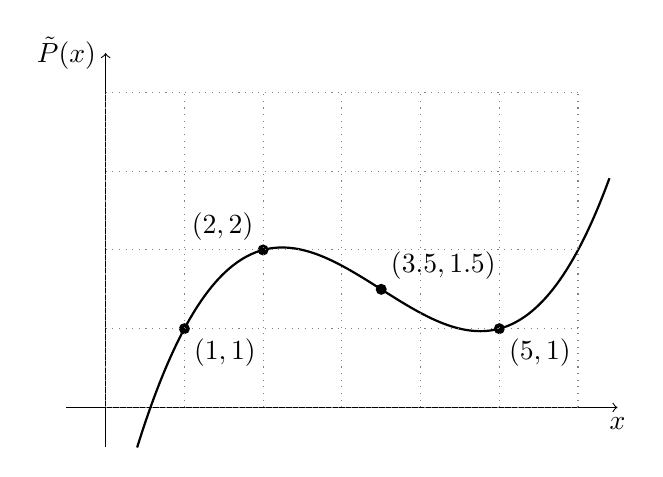
\begin{tikzpicture}
      \pgfmathsetmacro{\a}{2/15}
      \pgfmathsetmacro{\b}{-1.4}
      \pgfmathsetmacro{\c}{64/15}
      \pgfmathsetmacro{\d}{-2}
      
      \def\polynomial(#1){\a*(#1)^3 + \b*(#1)^2 + \c*(#1) + \d}
      
      \draw[->] (-0.5, 0) -- (6.5, 0) node[below] {$x$};
      \draw[->] (0, -0.5) -- (0, 4.5) node[left] {$\tilde P (x)$};
      
      \fill (1, 1) circle (2pt) node[below right] {$(1, 1)$};
      \fill (2, 2) circle (2pt) node[above left] {$(2, 2)$};
      \fill (3.5, 1.5) circle (2pt) node[above right] {$(3.5, 1.5)$};
      \fill (5, 1) circle (2pt) node[below right] {$(5, 1)$};
      
      \draw[thick, smooth, domain=0.4:6.4, samples=100] plot(\x, {\polynomial(\x)});
      
      \draw[gray, dotted] (0,0) grid (6,4);
    \end{tikzpicture}
    \caption{Le polynôme $\frac{2}{15}X^3 - \frac 7 5 X^2 + \frac{64}{15}X - 2$ est l'unique polynôme de degré $\leqslant 3$ passant par les points $\displaystyle \left((1, 1), (2, 2), \left(\frac 7 2, \frac 3 2 \right), (5, 1)\right)$}
  \end{figure}
  
\end{question_kholle}

\begin{question_kholle}
  [Soient $P$ à coefficients dans $\K$ et $a\in \K$. On a :
  \begin{equation}
    P = \sum_{n\in \N}\frac{\widetilde{P^{(n)}}(a)}{n!}(X-a)^n
  \end{equation}
  ]
  {Formule de Taylor dans $\K [X]$ (caractéristique nulle)}
  
  Considérons le prédicat $\PRIME (\cdot)$ défini sur $\N$ par :
  \[
  \PRIME (n ) \ :  \text{\textquotedblleft} \ \forall P \in \K _n[X], \ P = \sum_{k = 0}^n\frac{\widetilde{P^{(k)}}(a)}{k!}(X-a)^k \ \text{\textquotedblright}
  \]
  Initialisation : pour $n = 0 $, soit $P\in \K _0 [X]$. \\
  $\exists \ p_0 \in \K \ : \ P = p_0 X^0$ et $\sum_{k = 0}^0\frac{\widetilde{P^{(k)}}(a)}{k!}(X-a)^k = \frac{\widetilde{P^{(0)}}(a)}{1}X^0 = p_0 X^0$, donc $\PRIME (0)$ vrai. \\ \\
  Hérédité : Soit $n\in \N$ tel que $\PRIME (n)$. Soit $P\in \K _{n+1} [X]$. On a donc $\deg P' = \deg P -1 \leq n$ donc $\PRIME (n)$ s'applique à $P'$ :
  \[
  P' = \sum_{k = 0}^n\frac{\widetilde{P'^{(k)}}(a)}{k!}(X-a)^k = \left( \sum_{k = 0}^n\frac{\widetilde{P^{(k+1)}}(a)}{k!}\frac{(X-a)^{k+1}}{k+1} \right) ',
  \]
  donc :
  \[
  \left( P - \sum_{k = 0}^n\frac{\widetilde{P^{(k+1)}}(a)}{k!}\frac{(X-a)^{k+1}}{k+1} \right) ' = 0 \ \implies \ \exists \ \mu \in \K \ : \ P - \sum_{k = 0}^n\frac{\widetilde{P^{(k+1)}}(a)}{k!}\frac{(X-a)^{k+1}}{k+1} = \mu ,
  \]
  ainsi :
  \[
  P = \sum_{k = 0}^n\frac{\widetilde{P^{(k+1)}}(a)}{(k+1)!}(X-a)^{k+1} + \mu = \sum_{k = 1}^{n+1}\frac{\widetilde{P^{(k)}}(a)}{k!}(X-a)^{k} + \mu,
  \]
  donc en $a$ par $\ph _ a$ :
  \[
  \widetilde{P}(a) = \mu \ \implies \ P = \sum_{k = 1}^{n+1}\frac{\widetilde{P^{(k)}}(a)}{k!}(X-a)^{k} + \widetilde{P}(a) = \sum_{k = 0}^{n+1}\frac{\widetilde{P^{(k)}}(a)}{k!}(X-a)^{k},
  \]
  donc $\PRIME (n+1) $ vrai. Ainsi par théorème de récurrence sur $\N$, $\PRIME (n)$ est vrai pour tout $n\in \N$.
\end{question_kholle}

\begin{question_kholle}
  [Soit {$P \in \K[X]$}. Soit $a \in \K$.
  \begin{equation}
    a \text{ est une racine de } P \text{ de multiplicité au moins } m
    \iff \left\{ \begin{matrix}
      P(a) = 0  \\
      P'(a) = 0 \\
      \ldots    \\
      P^{(m-1)}(a) = 0
    \end{matrix} \right.
  \end{equation}
  \begin{equation}
    a \text{ est une racine de } P \text{ de multiplicité d'exactement } m
    \iff \left\{ \begin{matrix}
      P(a) = 0         \\
      P'(a) = 0        \\
      \ldots           \\
      P^{(m-1)}(a) = 0 \\
      P^{m}(a) \neq 0
    \end{matrix} \right.
  \end{equation}]
  {Caractérisation de la multiplicité d'une racine}
  
  \begin{enumerate}[label=$\bullet$]
    \item Supposons que $a$ est une racine de $P$ de multiplicité au moins $m$. \\
    Alors $\exists Q \in \K[X] : P = (X-a)^m Q$. D'après la formule de Leibniz, pour tout $k \in [\![0;m-1]\!]$,
    \begin{equation*}
      \begin{aligned}
        P^{(k)}
        & = \sum_{i=0}^{k} \binom{k}{i} \left( (X-a)^m \right) ^{(k-i)} Q^{(i)}       \\
        & = \sum_{i=0}^{k} \binom{k}{i} \frac{m!}{(m-(k-i))!} (X-a)^{m-(k-i)} Q^{(i)} \\
        & = \underbrace{ (X-a)^{(m-k)} }_{\substack{\text{c'est un bien un polynôme}  \\ \text{non constant car } k < m}} \sum_{i=0}^{k} \binom{k}{i} \frac{m!}{(m-(k-i))!} (X-a)^{i} Q^{(i)}
      \end{aligned}
    \end{equation*}
    Donc $\forall k \in [\![0;m-1]\!], P^{(k)}(a) = 0$.
    
    \item Supposons que $\forall k \in [\![0;m-1]\!], P^{(k)}(a) = 0$. \\
    Appliquons la formule de Taylor a.
    \begin{equation*}
      \begin{aligned}
        P & = \sum_{n \in \N} \frac{P^{(n)}(a)}{n!} (X-a)^n                                                   \\
        & = \sum_{n = 0}^{m-1} \underbrace{ \frac{P^{(n)}(a)}{n!} }_{=0} (X-a)^n + \sum_{\substack{n \in \N \\ n \geqslant m}} \frac{P^{(n)}(a)}{n!} (X-a)^n \\
        & = (X-a)^m \sum_{\substack{n \in \N                                                                \\ n \geqslant m}} \frac{P^{(n)}(a)}{n!} \underbrace{(X-a)^{n-m}}_{\in \K[X] \textit{ car } n - m \in \N}
      \end{aligned}
    \end{equation*}
    Donc $(X-a)^m | P$. Donc $a$ est racine de $P$ de multiplicité au moins $m$.
    
    \item Supposons que $a$ est une racine de $P$ de multiplicité exactement $m$. \\
    Nous pouvons appliquer le point précédent car la multiplicité est supérieur à $m$ : $\forall k \in [\![0;m-1]\!], P^{(k)}(a) = 0$. \\
    Par l'absurde, si $P^{(m)}(a) = 0$ alors le point précédent donne que $a$ a une multiplicité supérieur à $m + 1$ donc $m \geqslant m + 1$ ce qui est une contradiction. \\
    Par conséquent, $P^{(m)}(a) \neq 0$.
    
    \item Supposons $\forall k \in [\![0;m-1]\!], P^{(k)}(a) = 0$ et $P^{(m)}(a) \neq 0$. \\
    En reprenant le calcul précédent, pour $k = m$, en sachant que $(X-a)^{(m-k)} = X^0$,
    \begin{equation*}
      P^{(m)} = \binom{m}{0} \frac{m!}{0!} (X-a)^{0} P + \sum_{i=1}^{m} \binom{m}{i} \frac{m!}{i!} (X-a)^{i} Q^{(i)}
    \end{equation*}
    D'où $P^{(m)}(a) = m! \ Q(a)$ donc $Q(a) = \frac{P^{(m)}(a)}{m!}$. Donc $Q(a) \neq 0$. \\
    Par l'absurde, supposons que $(X-a)^{m+1} | P$. Alors $\exists R \in \K[X] : P = (X-a)^{m+1} R$. Donc $(X-a)^{m+1} R = (X-a)^m Q$ d'où $Q = (X-a) R$. Nous obtenons $Q(a) = 0$ ce qui est une contradiction avec $Q(a) = 0$. \\
    Donc $a$ est une racine de $P$ de multiplicité strictement inférieur à $m + 1$ et, d'après le point précédent, supérieur à $m$. Donc $a$ est une racine de $P$ de multiplicité exactement $m$.
  \end{enumerate}
\end{question_kholle}

\begin{question_kholle}
  []
  {Identification de $\K[X]$ à $\K [x]$, par l'injectivité de $\Phi$}
  Montrons que l'application $\Phi$ définie comme suit est injective :
  \[
  \Phi : \left|   \begin{array}{ccc}
    \K[X] & \longrightarrow & \mathcal{F}(\K, \K) \\
    P     & \longmapsto     & \widetilde{P}
  \end{array} \right..
  \]
  Soit donc $P\in \ker \Phi $, on a :
  \[
  \Phi (P)  = \widetilde{0} \ \implies \ \widetilde{P} = \widetilde{0} \text{ sur } \K \ \implies \ P = 0_{\K [X]},
  \]
  donc $\ker \Phi \subset \{ 0_{\K [X]} \}$. \\
  Réciproquement, on calcule l'image du polynôme nul par $\Phi$ :
  \[
  \Phi (0 _{\K [X]} ) = \widetilde{0},
  \]
  donc $0_{\K [X]} \in \ker \Phi$, ainsi on a l'égalité ensembliste et donc cela suffit.
\end{question_kholle}

\begin{question_kholle}
  [Les fonctions symétriques élémentaires $\displaystyle \left( \sigma_k \right)_{k \in [\![0;n]\!]}$ pour une famille $\displaystyle \left( x_k \right)_{k \in [\![1;n]\!]}$ sont définies par
  \begin{equation}
    \sigma_ k = \sum_{1 \leqslant i_1 < \ldots < i_k \leqslant n} \ \prod_{j=1}^{k} x_{i_j}
  \end{equation}]
  {Pour $P = (X-x_1)(X-x_2)(X-x_3)$, exprimer $x_1^3 + x_2^3 + x_3^3$ en fonction des fonctions symétriques élémentaires}
  
  Sous forme développée, $P = X^3 - (x1 + x_2 + x_3) X^2 + (x_1 x_2 + x_1 x_3 + x_2 x_3) X - x_1 x_2 x_3 = X^3 - \sigma_1 X^2 + \sigma_2 X - \sigma_3$. Comme $x_1, x_2, x_3$ sont racines de $P$, nous avons les trois égalité suivantes :
  \begin{equation*}
    \begin{aligned}
      0 = P(x_1) & = x_1^3 - \sigma_1 x_1^2 + \sigma_2 x_1 - \sigma_3 \\
      0 = P(x_1) & = x_2^3 - \sigma_1 x_2^2 + \sigma_2 x_2 - \sigma_3 \\
      0 = P(x_1) & = x_3^3 - \sigma_1 x_3^2 + \sigma_2 x_3 - \sigma_3
    \end{aligned}
  \end{equation*}
  En sommant ces trois équation,
  \begin{equation*}
    0 = x_1^3 + x_2^3 + x_3^3 - \sigma_1 (x_1^2 + x_2^2 + x_3^2) + \sigma_2 (x_1 + x_2 + x_3) - 3 \sigma_3
  \end{equation*}
  Cherchons la somme des carrés.
  \begin{equation*}
    \begin{aligned}
      (x_1 + x_2 + x_3)^2                       & = x_1^2 +  x_2^2 + x_3^2 + 2 x_1 x_2 + 2 x_1 x_3 + 2 x_2 x_3 \\
      \implies x_1^2 +  x_2^2 + x_3^2 + x_1 x_2 & = \sigma_1^2 - 2 \sigma_2
    \end{aligned}
  \end{equation*}
  Ainsi \begin{equation*}
    x_1^3 + x_2^3 + x_3^3 = \sigma_1^3 - 3 \sigma_1 \sigma_2 + 3 \sigma_3
  \end{equation*}
\end{question_kholle}

\begin{question_kholle}
  [Les sommes de Newton $(S_k)_{k\in\Z^*}$ pour une famille $(x_k)_{k \in \N^*}$ sont définies par (sous réserve d'existence pour $k<0$) :
  \begin{equation}
    S_k = \sum_{i=1}^{n} x_i^k
  \end{equation}]
  {Expression de $S_2$, $S_{-1}$ et $S_{-2}$ à l'aide des fonctions élémentaires symétriques.}
  
  \begin{equation*}
    \begin{aligned}
      \sigma_1^2   & = \left( \sum_{i=1}^{n} x_i \right)^2                                                                                      \\
      & = \underbrace{ \sum_{i=1}^{n} x_i^2 }_{S_2} + \ 2 \ \underbrace{ \sum_{1 \leqslant i < j \leqslant n} x_i x_j }_{\sigma_2} \\
      \implies S_2 & = \sigma_1^2 - 2 \sigma_2
    \end{aligned}
  \end{equation*}
  \begin{equation*}
    S_{-1} = \sum_{i=1}^{n} \frac{1}{x_i}
    = \frac{\displaystyle \sum_{i=1}^{n} \prod_{\substack{ j = 1 \\ j \neq i }}^{n} x_j }{\displaystyle \prod_{i=1}^{n} x_i }
    = \frac{\sigma_{n-1}}{\sigma_n}
  \end{equation*}
  \begin{equation*}
    \begin{aligned}
      S_{-2} & = \sum_{i=1}^{n} \frac{1}{x_i^2}                                                                                         \\
      & = \left( \sum_{i=1}^{n} \frac{1}{x_i} \right)^2 - 2 \sum_{1 \leqslant i < j \leqslant n} \frac{1}{x_i} \frac{1}{x_j}     \\
      & = \frac{\sigma_{n-1}^2}{\sigma_n^2} - 2 \frac{\displaystyle \sum_{1 \leqslant i < j \leqslant n} \prod_{\substack{ k = 1 \\ k \notin \{i,j\} }} \frac{1}{x_j} }{\sigma_n} \\
      & = \frac{\sigma_{n-1}^2 - 2 \sigma_{n-2}\sigma_n}{\sigma_n^2}
    \end{aligned}
  \end{equation*}
\end{question_kholle}
\end{document}
